\documentclass[a4paper]{article}
\usepackage[utf8]{inputenc}
\usepackage{hyperref}
\usepackage{listings}
\usepackage{graphicx}
\usepackage{biblatex}
\usepackage{amsmath}
\usepackage{amsfonts}
\usepackage{amssymb}

\addbibresource{sources.bib}
\graphicspath{{./media/}}

\title{Draft: Automating Output Evaluation}
\author{Jonas Mærsk Thye Kjellerup}
\date{\today}

\begin{document}

\maketitle
\newpage

%
% START COPY
%

\section{Self-similarity Matrices}\label{sec:theory-ssm}
A similarity matrix is used to analyse the similarity of two time series that consist of similar features. The matrix is described in terms of the similarity measure of its features $s : \mathcal{F} \times \mathcal{F} \rightarrow \mathbb{R}$, where $\mathcal{F}$ is a feature space. In turn the similarity matrix $S \in \mathbb{R}^{N \times M}$ is defined as follows, where $x$ and $y$ are time series:

\[ S(n,m)=s(x_n,y_m) \]

A self-similarity matrix (hereon abrreviated as SSM) is a similarity matrix, where both timeseries $x$ and $y$ are the same. Looking at the self-similarity data can be useful when trying to detect patterns and reptetion within data.

\begin{figure}[h]
    \center
    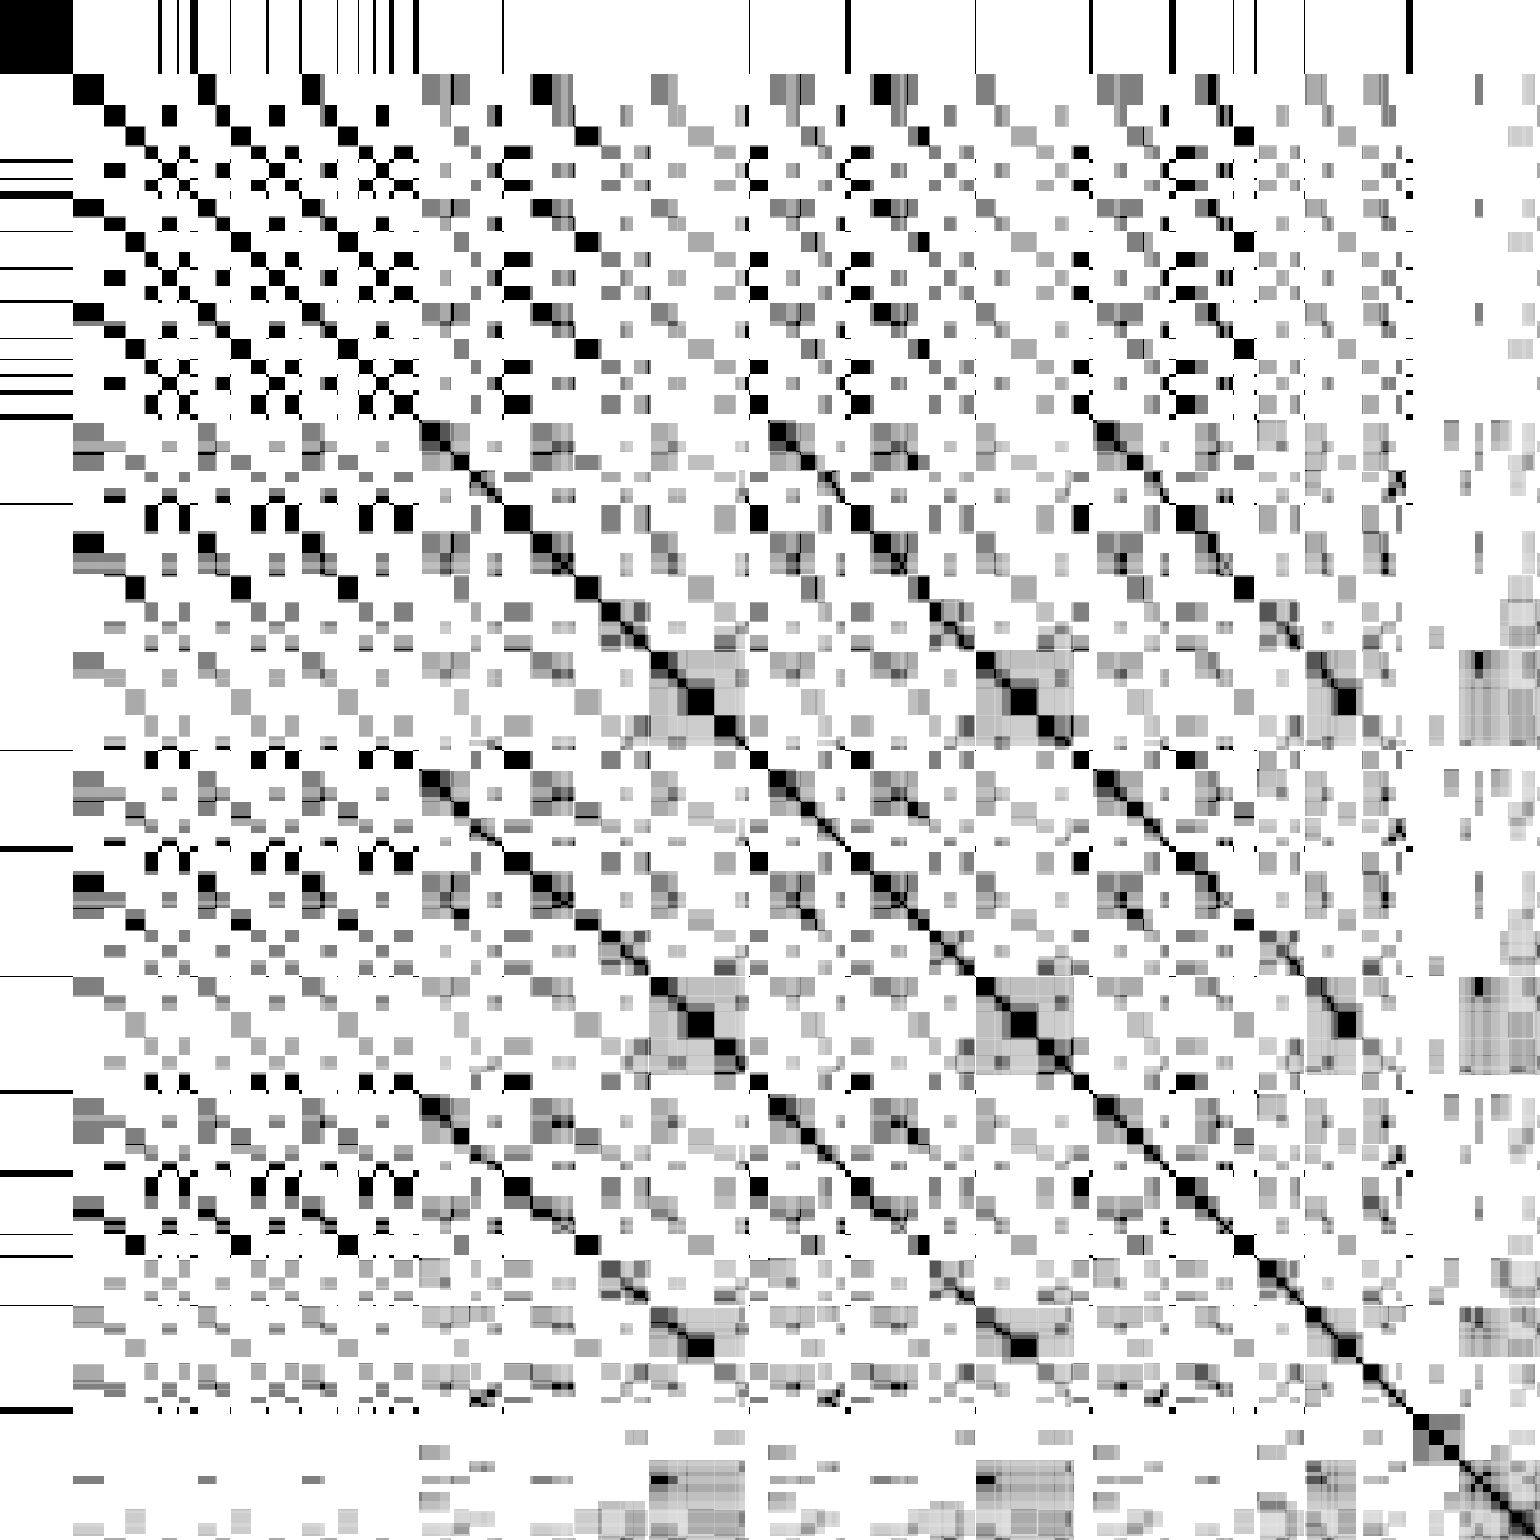
\includegraphics[width=3.5cm]{train_03.png}
    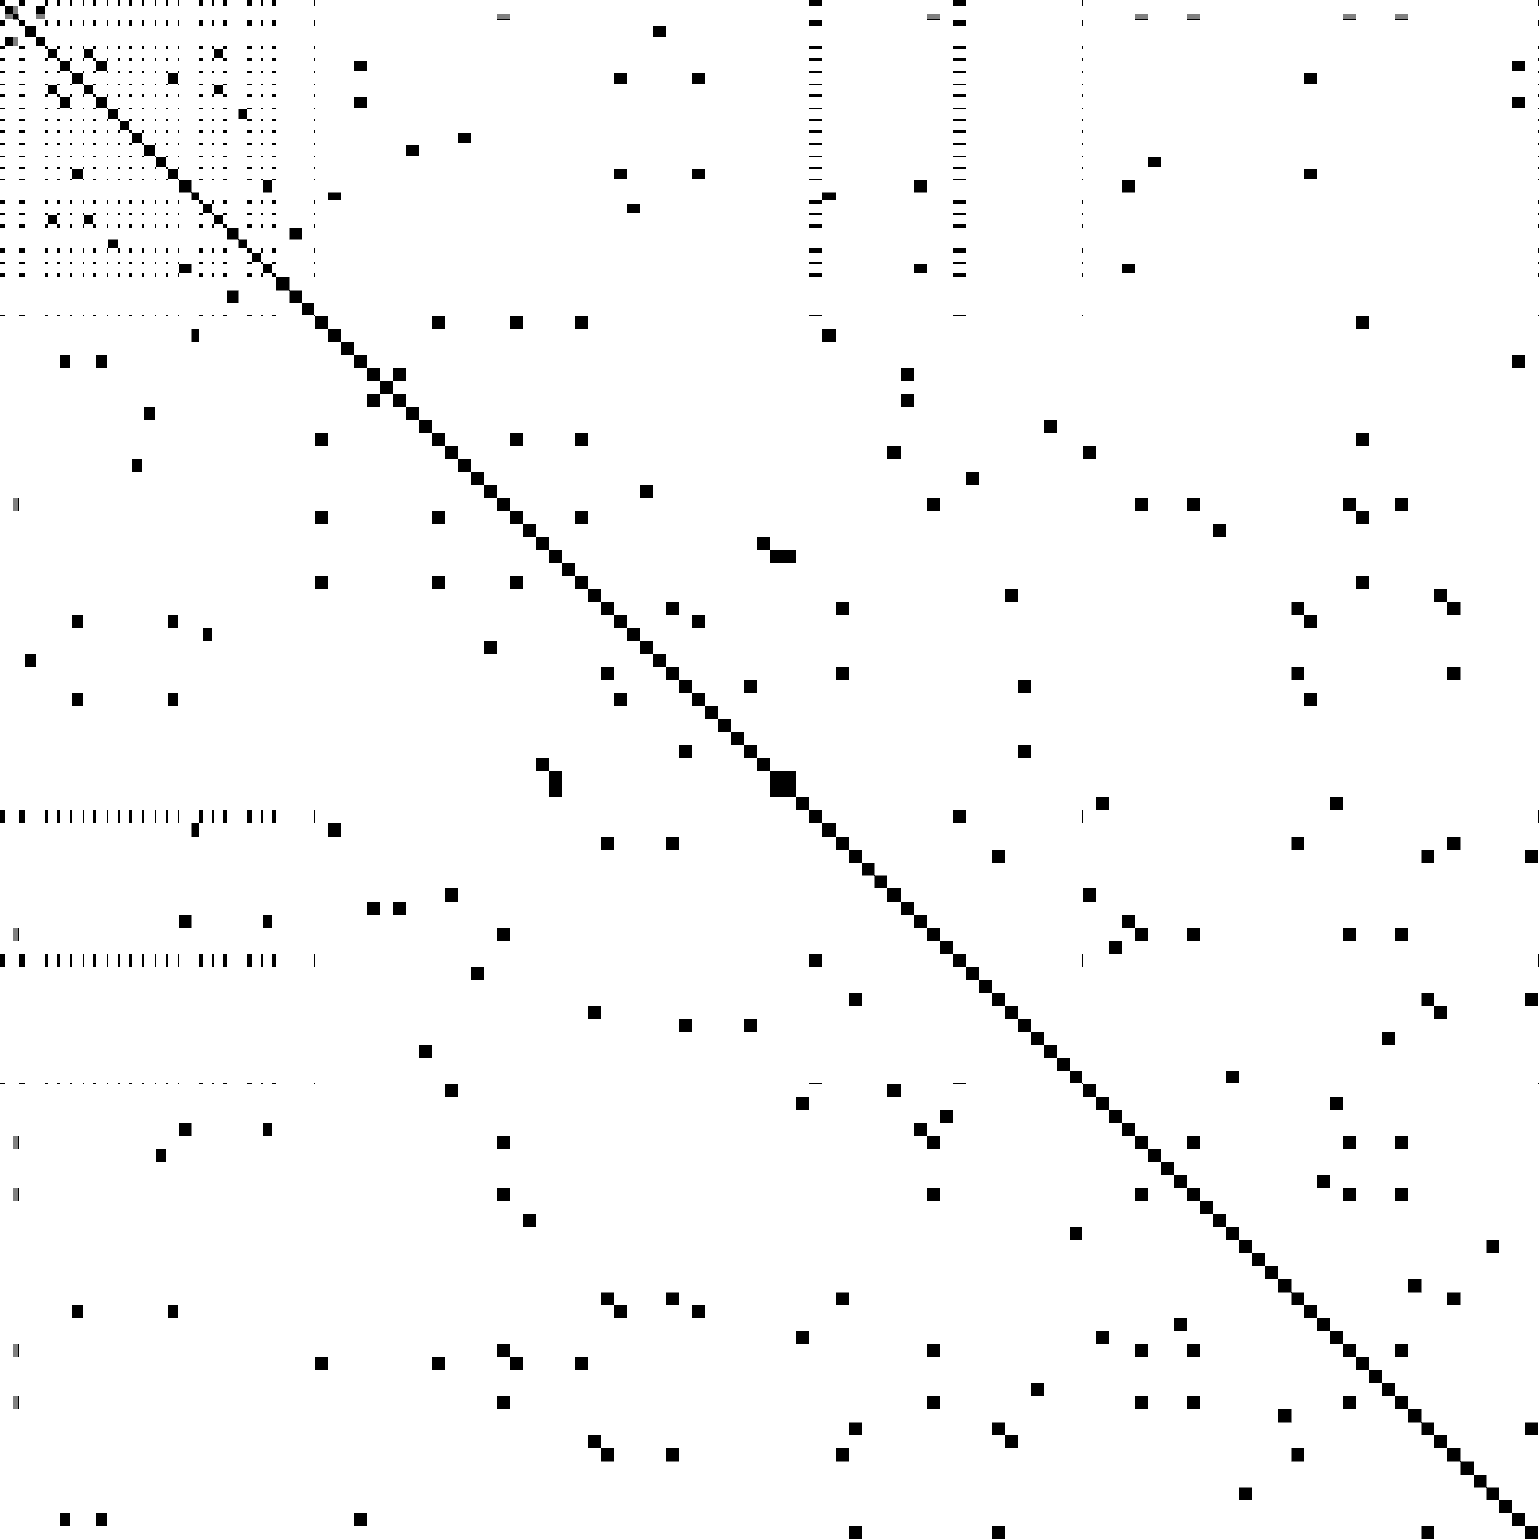
\includegraphics[width=3.5cm]{model_out_1.png}
    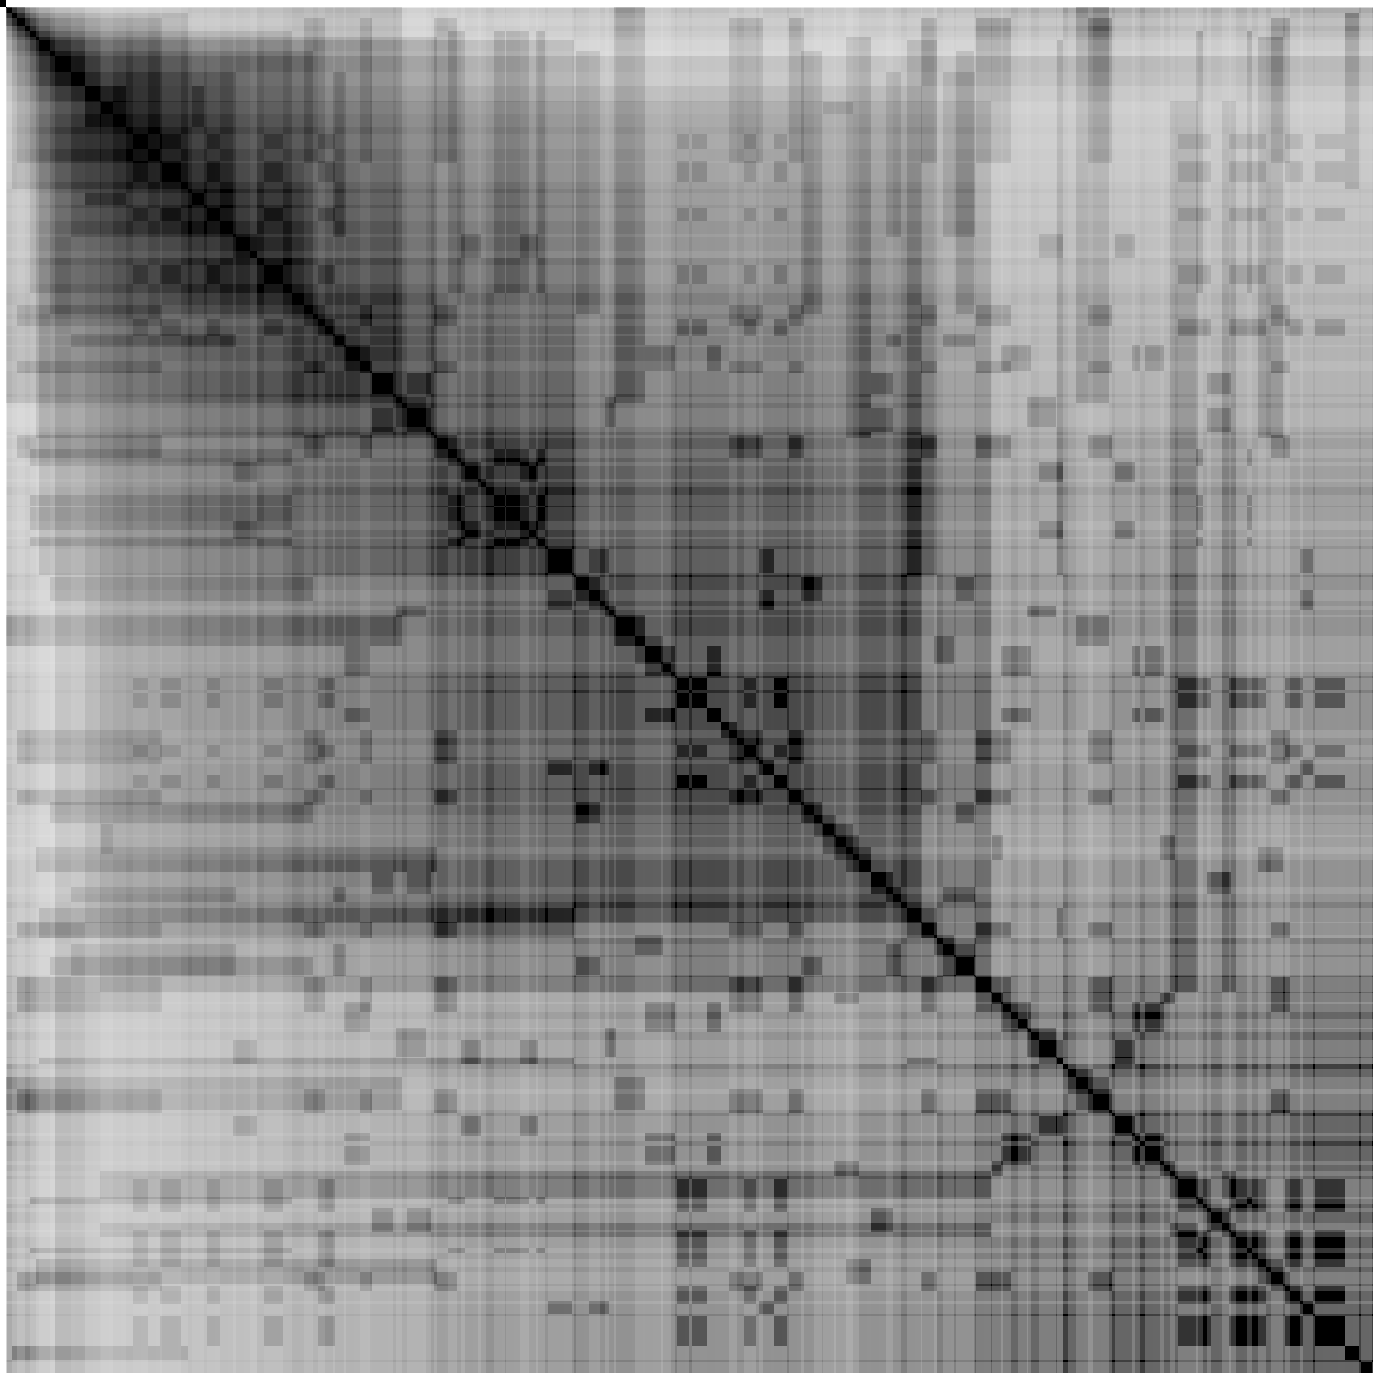
\includegraphics[width=3.5cm]{model_out_2.png}
    \caption{
        Visualisations of SSMs of three different datasets. The leftmost one being a MIDI file from the maestro dataset \cite{maestro}, and two other two being MIDI files output by a neural network.
    }
    \label{fig:ssm-comp}
\end{figure}

In figure \ref{fig:ssm-comp} it can be seen that the matrix is symmetric across the top-left/bottom-right diagonal, meaning that $S(x,y)=S(y,x)$. This is a result of the matrix being composed of two identical data series. This can be exploited when trying to store the digital representation of the matrix, in a computer program, by omitting either side of the matrix. This results in the matrix taking up memory equivalent to $N \cdot (N+1) \cdot \frac{1}{2}$ instead of $N^2$.

\section{Jaccard Index}\label{sec:theory-jaccard}

The Jaccard index is a measure of similarity between two sets. It is defined as the ratio between the intersection of two sets and the union of those sets. \cite{jaccard}

\[ J(A,B) = \frac{ A \cap B }{ A \cup B} \]

In the context of computer programming, it can be worth noting that a series of bits can be used to represent a finite set, where each bit represents whether a given element is present in the set. This allows for the substitution of the union and intersection operations in favor of the bitwise or and bitwise and operations, which are generally easier for a computer to compute.

\printbibliography

%
% END COPY
%

\end{document}